\documentclass{beamer}
\usepackage[T1]{fontenc}
\usepackage[utf8]{inputenc}
\usepackage{lmodern}
\usepackage[ngerman]{babel}

\usepackage{graphics}

\usepackage{amsmath}
\usepackage{booktabs}
\usepackage{listings}

\usepackage{dot2texi}
\usepackage{tikz}
\usetikzlibrary{arrows,shapes}
 \usetikzlibrary{matrix}
\usetikzlibrary{automata}

\usepackage{wrapfig}

\usetheme{Singapore}
\usecolortheme{dove}
\graphicspath{{images/}{../comics/}}

\newcommand{\xn}{\visible<2->{$\times$}}
\newcommand{\xj}{\visible<2->{$\checkmark$}}
\newcommand{\rd}[1]{\textcolor{red}{#1}}
\newcommand{\gn}[1]{\textcolor{green}{#1}}
\newcommand{\bl}[1]{\textcolor{blue}{#1}}

\newcommand{\hiddencell}[2]{\action<#1->{#2}}

\newcommand{\link}[2][blue]{\underline{\textcolor{#1}{#2}}} 	% \link{www.example.org} zeigt www.example.org in blau und unterstrichen
\renewcommand{\emph}[1]{\textit{\textcolor{blue}{#1}}}			% \emph{Test} zeigt Text in blau und kursiv
\newcommand{\warn}[1]{\textcolor{red}{#1}}			% \warn{Warning} zeigt Warning in rot und kursiv

\AtBeginSection[]
{
  \begin{frame}[plain]
    \frametitle{}
    {\footnotesize
      \tableofcontents[currentsection]
    }
  \end{frame}
}

\title{Grundbegriffe der Informatik}
\author{Patrick Niklaus}

\begin{document}
\begin{frame}
  \frametitle{Grundbegriffe der Informatik}
  \framesubtitle{8. Tutorium}
  \begin{description}
    \item \textbf{Name:} Patrick Niklaus
    \item \textbf{E-Mail:} patrick.niklaus@student.kit.edu
    \item \textbf{Nr:} 43
  \end{description}
\end{frame}

%\section{Übungsblatt}
%\begin{frame}
%  \frametitle{Anmerkungen zum letzten Übungsblatt}
%  \begin{enumerate}
%    \item Bla
%  \end{enumerate}
%\end{frame}


\section{Graphen}
\subsection{Motivation}
\begin{frame}[fragile]
  \frametitle{Was ist ein Automat?}
  \begin{tikzpicture}[]
    \begin{dot2tex}[styleonly,codeonly,neato]
      digraph G {
        d2ttikzedgelabels = true;
        node [style="state"];
        edge [lblstyle="auto",topath="bend left"];
        q_0 [style="state, initial"];
        q_0 -> q_1 [label=b]
        q_0 -> q_2 [label=a]
        q_1 -> q_1 [label=b,topath="loop above"];
        q_2 [style="state,accepting"];
      }
    \end{dot2tex}
  \end{tikzpicture}
\end{frame}

\subsection{Definitionen}
\begin{frame}[fragile]
  \frametitle{Endlicher Automat}
  \begin{definition}
    \begin{description}
      \item bla
    \end{description}
  \end{definition}\pause
  \begin{exampleblock}{Beispiele}
  \end{exampleblock}
\end{frame}

\subsection{Aufgaben}
\begin{frame}
  \frametitle{Aufgaben}
  \begin{exampleblock}{In Mengen M aus Studenten mit $|M| \leq 3$}
      Anweisung
      \begin{enumerate}
        \item Aufgabe
      \end{enumerate}
  \end{exampleblock}
\end{frame}


\section{Abschluss}
\subsection{Zusammenfassung}
\begin{frame}
  \frametitle{Was ihr jetzt wissen sollte.}
  \begin{enumerate}
    \item Was ist ein Mealy-Automat?
    \item Was ist ein Moore-Automat?
    \item Wie repräsentiert man diese Automaten grafisch?
  \end{enumerate}
\end{frame}

\subsection{xkcd}
\begin{frame}[plain]
  \begin{figure}
    \begin{center}
      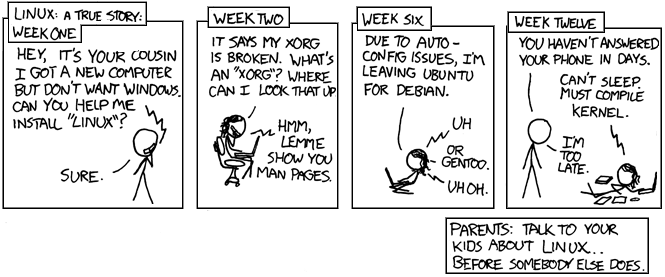
\includegraphics[width=300pt]{cautionary}
    \end{center}
    {\tiny This really is a true story, and she doesn't know I put it in my comic because her wifi hasn't worked for weeks.}
  \end{figure}
\end{frame}

\end{document}
